\section{Ground Handling in General}
This report will primarily focus on ground handling, but what exactly is this?

Ground handling is the work done to an aircraft from the time it lands until it takes off again (the handling of aircrafts on the ground). The actual ground handling consists of many different kinds of work; some ground handlers (un)load baggage, some clean the cabin and some fuel the aircraft amongst other important duties. The specific work done in a ground handling context will be described later in the report.

These ground handling duties are typically performed by ground handlers who are employed by either the airport or dedicated ground handling companies. In smaller airports, such as Aalborg Lufthavn, one employee can typically maintain various ground handling assignments, whereas in larger airports, like Københavns Lufthavn, each employee is typically assigned only one job. Likewise in smaller airports, the airport itself is typically in charge of the ground handling staff, where larger airports usually hire ground handling companies.

The time ground handling takes for an aircraft varies greatly. The amount of ground handlers and equipment assigned to an aircraft is usually dependent on the time before the aircraft has to take off again. Some aircrafts have a lot of ground time, and thus the workload is spread out over a long period of time, whereas others have to take off almost immediately, and the work is prioritized highly and a lot of workers are assigned that aircraft.


A rough visualization of the time it takes for aircraft to be handled can be seen here:
\begin{figure}[H]
\centering
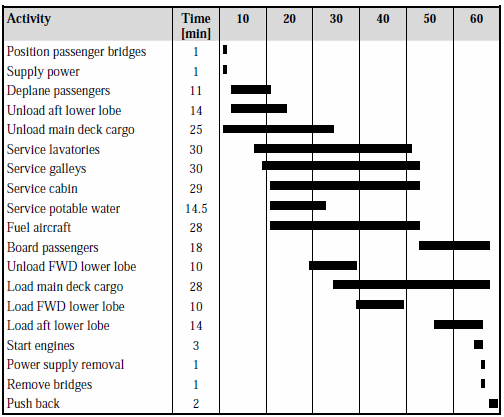
\includegraphics[width=300px]{Grafik/timetable}
\caption{A general timetable of a turnaround af Boeing 737-800.}
\label{timetable}
\end{figure}